\documentclass{article}
\usepackage{graphicx}

\begin{document}

\title{CS181 Spring 2016 Practical 1}
\author{Robert J. Johnson | Dinesh Malav | Matthew McKenna}


\maketitle

\begin{abstract}
The Harvard Clean Energy Project has been investigating the features and characteristics of organic photovoltaic molecules in an effort to create carbon-based solar cells. Density Functional Theory (DFT) has been traditionally used to estimate the energy difference from the highest occupied molecular orbital (HOMO) and the lowest unoccupied molecular orbital (LUMO). DFT calculations are computationally expensive, and thus we have developed an [insert method here] algorithm to predict the HOMO-LUMO gap based on the chemical structure of an organic photovoltaic molecule. Using [insert method here] the HOMO-LUMO gaps of our test data were predicted with a RMSE of [insert final score here].
\end{abstract}

\section{Technical Approach}
The approach that our team took was an iterative one. Very early on in the process, our team established that we had relatively little domain knowledge of organic chemistry. Thus, we attempted to implement various proven techniques and algorithms such as Ridge Regression, Random Forest Regression, Bayesian Linear Regression, Neural Networks, and Support Vector Machines. However, these were not able to beat the RMSE baselines set by the example OLS (RMSE = 0.29846) and Random Forest Regression (RMSE = 0.27207) established by the teaching staff. A different technique was needed.\\\\
It became abundantly clear that feature engineering was the key to improving the model. Using the RDKit package in Python, we were able to extract some basic information regarding the SMILEs molecules. These were basic yet important pieces of information regarding a molecule: the total number of atoms, the total number of bonds, and the molecular weight of the molecule. Undoubtedly, knowledge of specific types of bonds and chemical rings may have improved the analysis here, but for the time being, these factors were determined to be enough to improve on the model.\\\\

\begin{figure}[h]
\centering
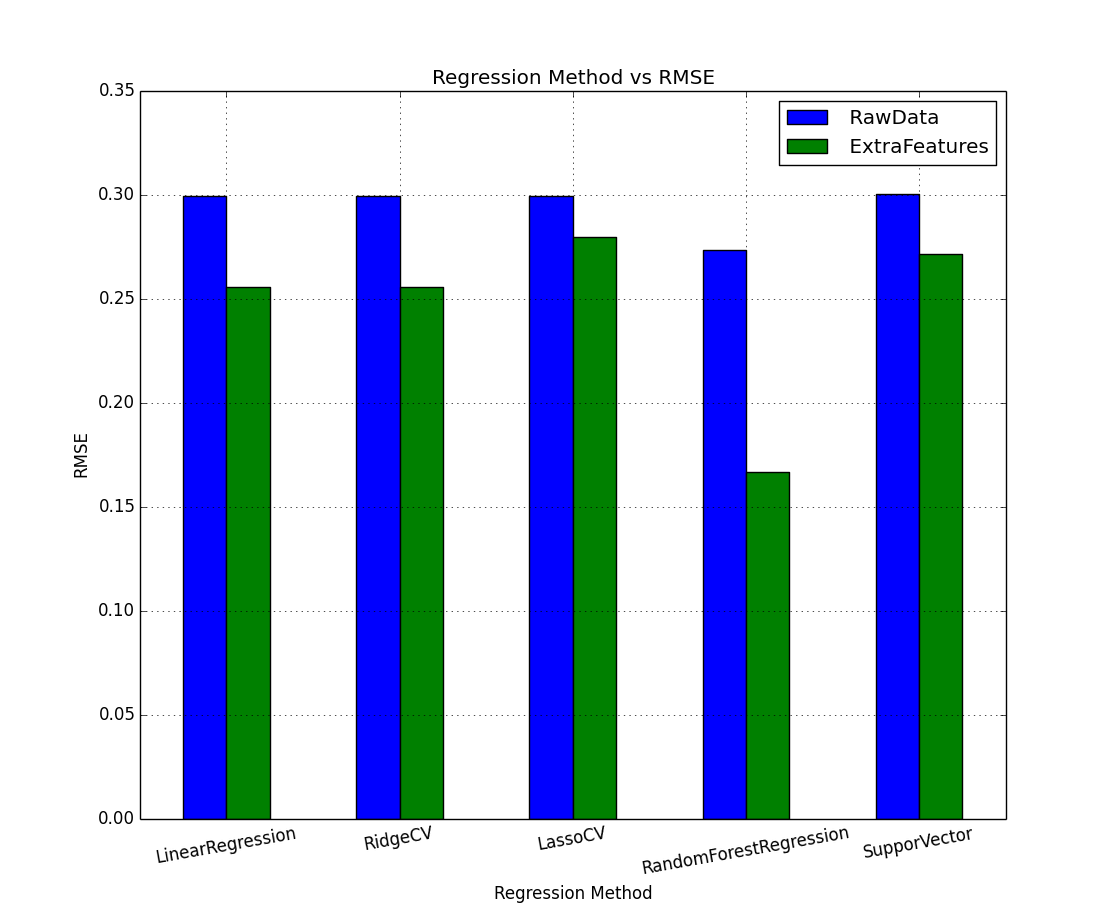
\includegraphics[width=0.8\textwidth]{method_selection}
\caption{Regression Method vs RMSE}
\label{fig:method_selection}
\end{figure}

\begin{center}
\begin{table}
\centering
\begin{tabular}{ |c|c| } 
 \hline
num of estimators & RMSE \\
 \hline
 10 &  0.166937109962 \\ 
 100 & 0.165886177921 \\ 
 200 & 0.165816557416 \\ 
 \hline
\end{tabular}
\caption{Changing Random Forest Regression parameters}
\label{table:1}
\end{table}
\end{center}

\section{Results}
The model that we ultimately chose to tune was the Random Forest Regressor. Our training data contained 256 features, of which we were not familiar with either their function or how they impacted
\section{Discussion}



\end{document}
